\chapter{Spin transport in long-range anisotropic Heisenberg model\label{chap:spin_transport}}
\thispagestyle{chapterBeginStyle}

After all the technicalities of the previous chapter, we are finally ready to study spin transport in
the long-range anisotropic Heisenberg model. The main motivation of this investigation is the fact that this model admits 
two limits exhibiting ballistic spin transport (cf. Fig.~\ref{fig:spin_transport}), namely the free particles
with nearest-neighbor hopping for \(\alpha\to \infty,\; \Delta = 0\) and the Haldane-Shastry
model with \(J_{\mathrm{HS}(r)} = J \sin^2\left(\pi/L\right)/\sin^2\left(\pi r/L\right)\)
 for \(\alpha = 2\)~\autocite{Haldane1988,Shastry1988}. In the latter case, this limit is only strictly valid
 in the thermodynamic limit, since \(\sin^{-2}\left(r/L\right)\propto r^{-2}\) for \(r \ll L\).
 In both of these limiting models the spin current 
\(j^{\sigma}\) commutes with the Hamiltonian and thus is strictly conserved. Hence, even though
the Hamiltonian~\eqref{eq:long_range} is not integrable for arbitrary \(\alpha\), one could suspect
that it will be \textit{nearly integrable}, in the sense described in the introduction, and support
interesting transport properties. Using spin density expansion and linear response theory
of optical conductivity, in this chapter we will show that this is indeed the case and the spin transport is \textit{quasibalistic} along a sharp
line in the parameter space \(\Delta \simeq \exp(- \alpha + 2)\), which continuously connects the two limiting
cases mentioned above.

Results described in this chapter were first presented in chapters II and III of ~\textcite{Mierzejewski2023}.

\begin{figure}[htbp]
    \centering
    \begin{tikzpicture}[scale=1.5]
      % \colorlet{col1}{blue!30}
      \colorlet{col1}{wppt!50}
    
     \begin{scope}[smooth,draw=gray!20,y=0.3989422804cm]
          \filldraw[fill=col1] plot[id=f1, domain=-1.5:1.5,samples=100] function {6*exp(-6*x*x)};
          \draw[black] plot[id=f2,domain=-1.5:1.5,samples=100]
              function {6*exp(-6*x*x)};
      \end{scope}
      \draw[->] (-1.5,0) -- (1.5,0) node [right] {$x$};
      \draw[->] (-1.5,0) -- (-1.5,2.5) node [midway,rotate=90,yshift=6pt] {spin density};
      \draw[<->] (-0.37,1) -- (0.37,1) node [midway, yshift=6pt] {$\gamma$};
    
      \begin{scope}[smooth,draw=gray!20,y=0.3989422804cm]  
        \draw[wppt] plot[id=f3,domain=2.35:5.35,samples=100] function {0.7};    
        \draw[wppt] plot[id=f4,domain=2.35:5.35,samples=100] function {x};    
        \draw[wppt] plot[id=f5,domain=2.35:5.35,samples=100] function {sqrt(x)};    
      \end{scope}  
      
      \draw[->] (2.35,0) -- (5.35,0) node [right] {$t$};
      \draw[->] (2.35,0) -- (2.35,2.5) node [right] {$\gamma$};
      \node[draw=none] at (3.35,1.6) {$\gamma \propto t$};
      \node[draw=none] at (3.45,0.95) {$\gamma \propto \sqrt{t}$};
      \node[draw=none] at (3.6,0.4) {$\gamma = const$};
      \node[draw=none] (localized) at (6,0.3) {localized};
      \node[draw=none,above of=localized,node distance=27pt] (diffusive) {diffusive};
      \node[draw=none,above of=diffusive,node distance=45pt] (ballistic) {ballistic};
    \end{tikzpicture}  
    \caption{Illustration of different types of transport. On the left panel, we have some initial spin
    density characterized by width \(\gamma\). On the right panel, we have the dependence of \(\gamma\)
    on time in three different cases.}
    \label{fig:spin_transport}
  \end{figure}
  
  \section{Spin density expansion}

  Taking inspiration from experimental studies of cold atoms~\autocite{Joshi2022, Ronzheimer2013, Vidmar2013, Neyenhuis2017},
  we consider an initial state in the form of a spin domain wall
  \begin{equation}
    \ket{\psi(0)} = \ket*{\underbrace{\uparrow\uparrow\uparrow\uparrow\uparrow}_{x}
    \underbrace{\downarrow\downarrow\downarrow\ldots\downarrow}_{L-x}},\; x = 5
  \end{equation}
and study the dynamics of spin expansion by measuring the time dependence of the magnetization profile
\(M_{\ell}(t) = \matrixel{\psi(t)}{\Sz_{\ell}}{\psi(t)}\). Such a product state initial configuration is desirable for two reasons.
First, it is relatively accessible in experiments, e.g. using higher-order optical Stark shifts to rotate individual
spins~\autocite{Lee2016}. Second, from the theoretical point of view, by assuming open boundary conditions and
choosing \(x = 5\), we localize the domain wall close to the edge of the system, which allows us to avoid finite-size effects
for longer times. Moreover, the dynamics generated by the Hamiltonian~\eqref{eq:long_range} conserve the total magnetization
and hence we can restrict ourselves to the subspace of states with just \(5\) spins up. This considerably reduces
the dimensionality of the problem and allows us to study systems as large as \(L=45\) with
\(\binom{45}{5} \approx 1.2 \times 10^6\) states, characterized by the total magnetization \(M_{\mathrm{tot}} = -35/2\).
To put this into perspective, the full Hilbert space of such system
has dimension \(2^{45}\) which is \(O(10^7)\) larger and thus completely inaccessible without additional techniques.

For the time evolution, we use the Krylov propagator introduced in detail in the previous chapter.
A sample magnetization profile obtained for \(\alpha = 3.5\) and \(\Delta = 1.0\) is shown in 
Fig.~\ref{fig:magnetization_profile}.
\begin{figure}[htbp]
  \centering
  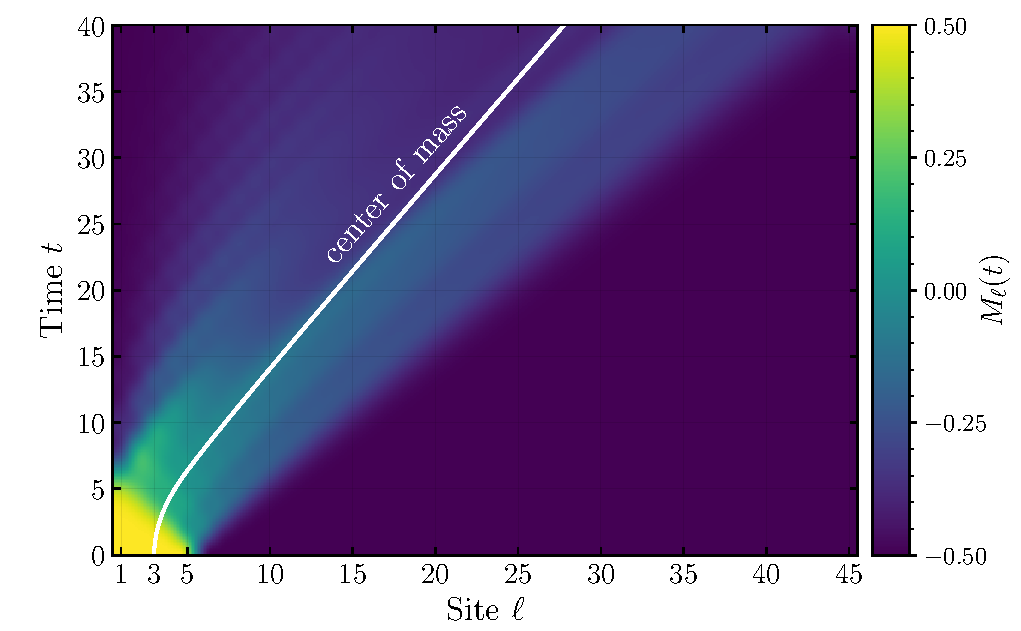
\includegraphics[width=0.8\linewidth]{Figures/magnetization.pdf}
  \caption{Time dependence of magnetization profile \(M_{\ell}(t)\) for \(\alpha = 3.5\) and \(\Delta = 1.0\).
  The evolution of the center of mass, initially at \(r_{\text{cm}}(t=0)=3\), is marked by a white line.}
  \label{fig:magnetization_profile}
\end{figure}
% \newpage
In order to quantitatively investigate the spin transport in this setup, we introduce the so-called
\textbf{center of mass}, defined as the first density moment of the magnetization profile  
\begin{equation}
  r_{\text{cm}}(t) = \frac{\sum_{\ell=1}^{L} \ell \left(M_{\ell}(t)+1/2\right)}
  {\sum_{\ell=1}^{L} \left(M_{\ell}(t) + 1/2\right)} = 
\frac{\sum_{\ell=1}^{L} \ell \left(M_{\ell}(t)+1/2\right)}
  {M_{\mathrm{tot}} + L/2}
  \label{eq:center_of_mass} 
\end{equation}
In Fig.~\ref{fig:magnetization_profile}, an example of time evolution of center of mass is shown. Examining \(r_{\text{cm}}(t)\)
calculated for two values of \(\Delta = 0.2,\;0.5\) and various values of \(\alpha \in \{2.0,2.5,\ldots,5.0\}\)
(cf. Fig.~\ref{fig:center_of_mass}), we observe a first hint of non-trivial transport properties of the model, namely
non-monotonic dependence of \(r_{\text{cm}}(t)\) on \(\alpha\). 

\begin{figure}[htbp]
  \centering
  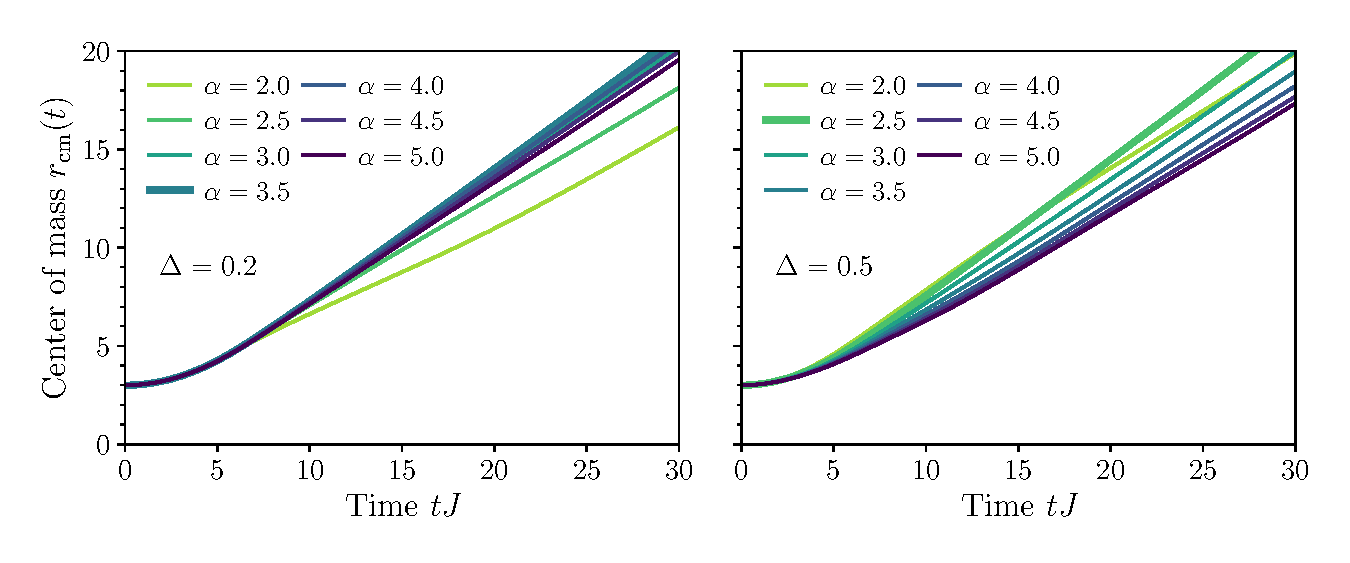
\includegraphics[width=0.9\linewidth]{Figures/center_of_mass.pdf}
  \caption{Time dependence of the center of mass \(r_{\text{cm}}(t)\) for \(\Delta = 0.2\) (left panel) and \(\Delta = 0.5\)
  (right panel) and various values of interaction decay \(\alpha\). The line corresponding to the fastest-moving center of mass
  is thicker than the rest.}
  \label{fig:center_of_mass}
\end{figure}

To see this better, in Fig.~\ref{fig:velocity} we look at the velocity
obtained from the time derivative of the center of mass
\begin{equation}
  {\nu}_{\text{cm}}(t) = \dv{r_{\text{cm}}(t)}{t}.
  \label{eq:velocity}
\end{equation}
\begin{figure}[htbp]
  \centering
  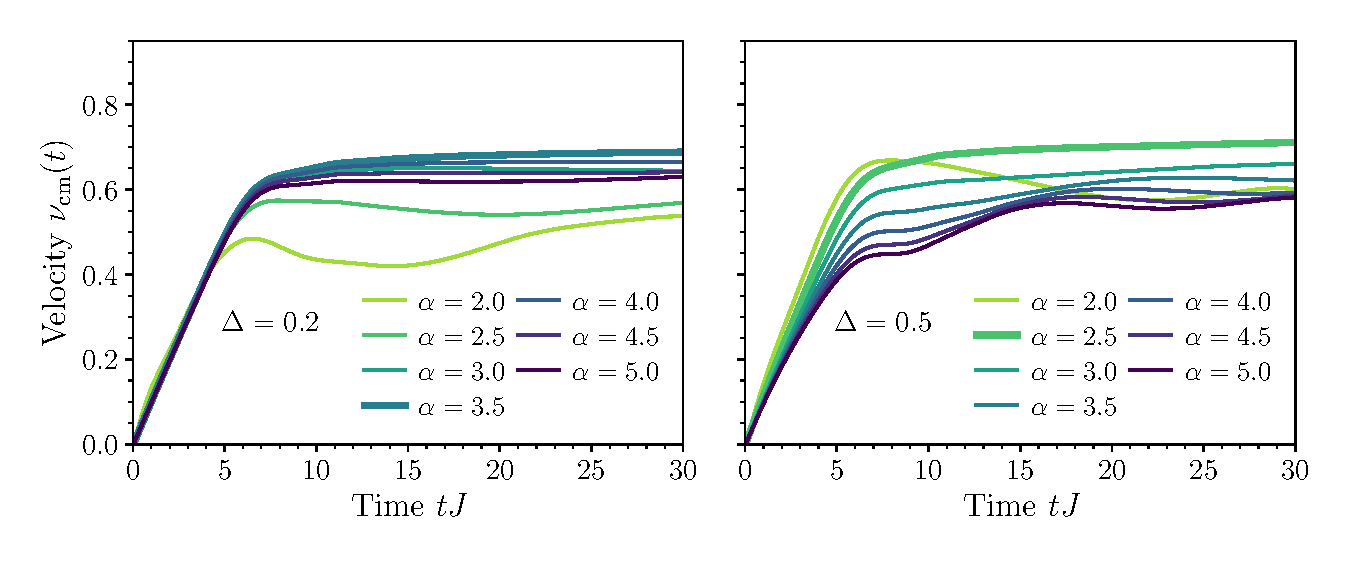
\includegraphics[width=0.9\linewidth]{Figures/velocity.pdf}
  \caption{Time dependence of the velocity \(\nu_{\text{cm}}(t)\) for \(\Delta = 0.2\) (left panel) and \(\Delta = 0.5\)
  (right panel) and various values of interaction decay \(\alpha\). The line corresponding to the largest velocity
  is again thicker than the rest.}
  \label{fig:velocity}
\end{figure}
We observe that for both values of \(\Delta\), there is a clear maximum of the velocity of the expansion
at some intermediate value of \(\alpha\). Investigating further the dependence of velocity on the parameters
of the model, we calculate the average velocity \(\bar{\nu}_{\text{cm}}\) on the interval \(t\in\left[20,30\right]\)
and plot it as a function of \(\alpha\) for various values of \(\Delta\)
(cf. left panel of Fig.~\ref{fig:optimal_velocity}).
The non-monotonic behavior is now evident, as for a fixed \(\Delta\), there exists a value of 
\( \alpha = \alpha_{\nu_{\mathrm{max}}}(\Delta) \),
such that the average velocity has a maximum (for \(\Delta = 0.0\) the optimal \(\alpha\) is shifted to infinity).
Equivalently, for each \(\alpha\) there exists an optimal value of \(\Delta = \Delta_{\nu_{\mathrm{max}}} (\alpha)\).

In the right panel of Fig.~\ref{fig:optimal_velocity} we look at the dependence of average velocity on both
parameters of the model. Moreover, we superimpose the points corresponding to the
optimal anisotropies \(\Delta_{\nu_{\mathrm{max}}} (\alpha)\). Curiously, these points
seem to lie very close to an exponential curve, given by \(\Delta_{\mathrm{O}} = \exp\left(-\alpha + 2\right)\).
Furthermore, as seen in the left panel, the average velocity is approximately constant for \(\alpha \geq 2\) and equal to
\(\bar{\nu} \simeq J/\sqrt{2}\) along this line. Such velocity is a characteristic of ballistic
transport in the nearest neighbors free-fermion model~\autocite{Vidmar2013, Langer2012},
corresponding via Jordan-Wigner transformation to our model with \(\alpha \to \infty\) and \(\Delta = 0\).
Therefore, we suspect that the optimal line \(\Delta_{\nu_{\mathrm{max}}} (\alpha)\), present in this interacting
system and indicating \textbf{quasibalistic} transport, is a transient remnant of the transport properties of the free fermions.

\begin{figure}[htbp]
  \centering
  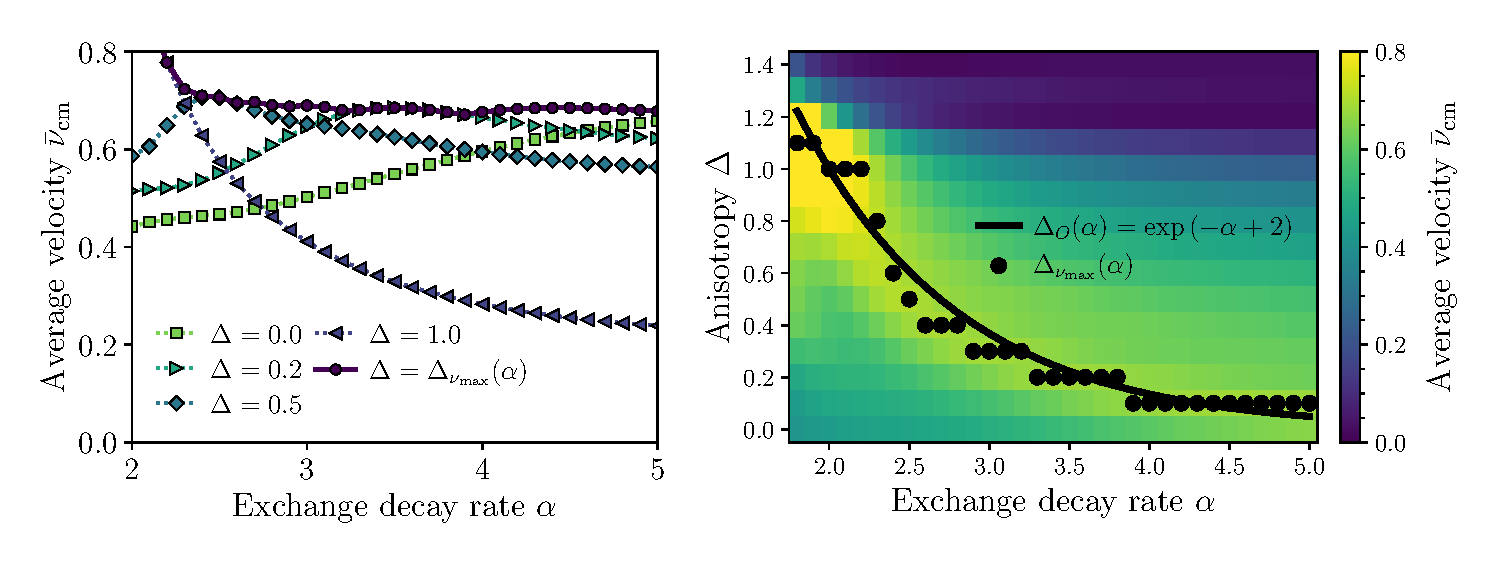
\includegraphics[width=\linewidth]{Figures/optimal_velocity.pdf}
  \caption{Left panel: average velocity \(\bar{\nu}_{\text{cm}}\) as a function of \(\alpha\) for various values of \(\Delta\).
  Right panel: heatmap of the average velocity \(\bar{\nu}_{\text{cm}}\) as a function of \(\alpha\) and \(\Delta\). The points
  corresponding to the optimal anisotropies \(\Delta_{\nu_{\mathrm{max}}} (\alpha)\) are marked with black dots, while the solid line
  indicates the optimal line \(\Delta = \Delta_{\mathrm{O}} = \exp\left(-\alpha + 2\right)\).}
  \label{fig:optimal_velocity}
\end{figure}


\section{Optical conductivity}

In this section, we approach the problem of spin transport in the long-range Heisenberg model from the
perspective of \textbf{linear response theory}. We study the \textbf{optical conductivity}
\footnote{The optical conductivity is also known as the spin conductivity.} \(\sigma(\omega)\) of the model,
which is a measure of the response of the system to an external electromagnetic field. 
In the linear response regime, the optical conductivity is given by the Kubo formula, which
for infinite temperature reads
\begin{equation}
  \sigma(\omega) = \frac{\pi}{L \mathcal{Z}} \sum_{n,m} \abs{\mel{n}{j^{\sigma}}{m}}^2 \delta(\omega - \epsilon_m + \epsilon_n)
  \label{eq:kubo}
\end{equation}
where \(\mathcal{Z}\) is the number of states in the Hilbert space, \(L\) is the system size and \(j^{\sigma}\) is the spin
current operator~\eqref{eq:spin_current}, derived in Chapter~\ref{chap:intro}.
For the derivation of the Kubo formula and the optical conductivity, see Appendix~\ref{app:opt_cond}.
As the sum in Eq.~\eqref{eq:kubo} runs 
uniformly over all many-body eigenstates \(H \ket{n} = \epsilon_n \ket{n}\) of the Hamiltonian, this quantity
probes the whole eigenspectrum. Equation~\ref {eq:kubo} suggests a simple numerical procedure for calculating
the optical conductivity. First, one needs to diagonalize the Hamiltonian \(H\) and obtain the eigenstates
\(\ket{n}\) and eigenvalues \(\epsilon_n\). Then, one needs to calculate the matrix elements of the spin current operator
\(\mel{n}{j^{\sigma}}{n}\) between all pairs of eigenstates. Finally, the optical conductivity is obtained by
summing over all pairs of eigenstates, weighted by the corresponding matrix elements and the \(\delta\) function.
It is only the last step that requires some care, as the \(\delta\) function is not a regular function and
would require some binning of the discrete spectrum. We avoid this, by instead considering the
\textbf{integrated conductivity}
\begin{equation}
  I(\Omega) = \frac{1}{\mathcal{S}_{\mathrm{tot}}} \int_{-\Omega}^{\Omega} \dd{\omega} \sigma(\omega) = 
  \frac{\pi}{L \mathcal{Z} \mathcal{S}_{\mathrm{tot}}} \sum_{n,m} \abs{\mel{n}{j^{\sigma}}{m}}^2 \theta(\Omega- \abs{\epsilon_m - \epsilon_n})
  \label{eq:integrated_conductivity}
\end{equation}
where \(\theta(x)\) is the Heaviside step function and  \(\mathcal{S}_{\mathrm{tot}}\) is the sum rule
\begin{equation}
  \mathcal{S}_{\mathrm{tot}} = \int_{-\infty}^{\infty} \dd{\omega} \sigma(\omega) = \frac{\pi}{L \mathcal{Z}} \sum_{n,m} \abs{\mel{n}{j^{\sigma}}{m}}^2
\end{equation}
It is easy to see that the integrated conductivity \(I(\Omega)\) is a regular function of \(\Omega\), and
contains the information about the fraction of the spectral weight contained in the frequency window 
\(\left[-\Omega,\Omega\right]\).
Equation~\eqref{eq:integrated_conductivity} is now straightforward to evaluate numerically.

We evaluate the integrated conductivity~\eqref{eq:integrated_conductivity} for the long-range Heisenberg model
with periodic boundary conditions, and system sizes up to \(L=20\). We also restrict the calculations to the
subspace of zero total magnetization, i.e. the largest sector with \(\binom{L}{L/2}\) states. Leveraging
the periodic boundary conditions, we perform the calculations separately for each momentum sector and then
add the results together.

\begin{figure}[htbp]
  \centering
  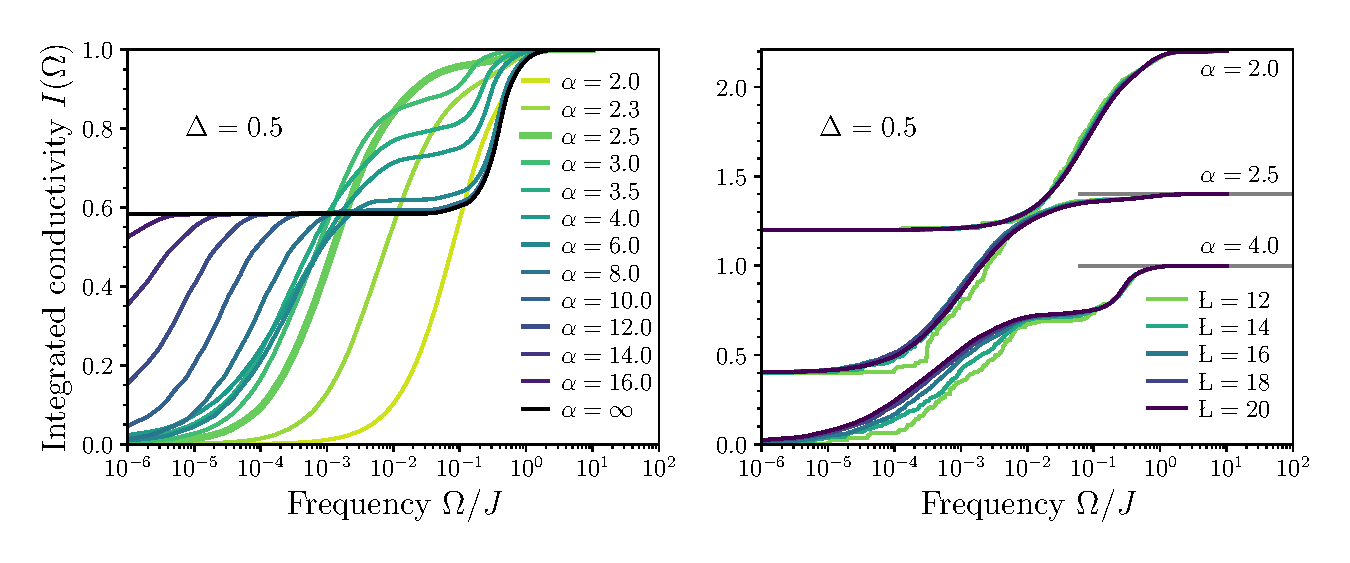
\includegraphics[width=\linewidth]{Figures/optical_conductivity.pdf}
  \caption{Left panel: Integrated conductivity \(I(\Omega)\) as a function of frequency window \(\Omega\) for various values of \(\alpha\)
  and \(\Delta = 0.5\). The thicker line denotes the result for optimal decay parameter \(\alpha\). Right panel: Size dependence
  of the integrated conductivity \(I(\Omega)\) for \(\alpha = 2.0, \; 2.5,\; 4.0\) and \(\Delta = 0.5\),
  illustrating the effects of finite size. For clarity, we added a vertical shift to distinguish the curves for different
  decay parameters.}
  \label{fig:optical_conductivity}
\end{figure}

Looking at the left panel of Fig.~\ref{fig:optical_conductivity}, we observe that the integrated conductivity
for \(\alpha \to \infty\) is exhibiting a \textbf{Drude peak} behavior at \(\Omega \to 0\), and a distinct 
incoherent (regular) spectrum for \(0.1 \lesssim \Omega / J \lesssim 1.0\), which is consistent with the results
for the nearest neighbor Heisenberg model~\autocite{Prelovsek2021}. As \(\alpha\) is decreased 
(the range of the interactions increases), but remains \(\alpha \gtrsim 10\), the Drude peak
becomes suppressed, while the regular part of the spectrum is still more or less the same.
However, an interesting feature appears in the spectrum for \(\alpha \lesssim 10\), namely
the incoherent part starts shifting towards lower frequencies. For anisotropy \(\Delta = 0.5\),
this behavior is most pronounced for \(\alpha = 2.5\), where the integrated conductivity
is \(I(\Omega)\simeq 1 \) for all \( \Omega/J < 0.01\), which means that most of the spectral weight
is contained in the frequency window \(\left[-0.01,0.01\right]\). This in turn implies ballistic-like 
spin transport for extremely long times up to \(tJ \simeq 100\), similar to the case of noninteracting particles,
as there we have \(\sigma(\omega) \propto \delta(\omega) \implies I(\Omega) = 1\) for \(\Omega > 0\). Furthermore,
we once again observe some kind of non-monotonic behavior, as decreasing the decay parameter
beyond \(\alpha \approx 2.5\) shifts the incoherent part of the spectrum back towards higher frequencies.

To quantitatively investigate this effect across the parameter space, in Fig.~\ref{fig:I_cond_heatmap}
we present heatmaps of the integrated conductivity \(I(\Omega)\) on the \((\alpha ,\Omega)\) plane, 
for different values of the anisotropy \(\Delta\). Moreover, with a solid black line we denote the
the value \(\Omega = \Omega^{\ast}\), for which the integrated conductivity is \(I(\Omega^{\ast}) = 0.9\),
i.e. 90\% of the sum rule \(S_{\mathrm{tot}}\).


As in the case of average velocity during a spin expansion experiment, 
for every value of \(\Delta\), we can find a value of \(\alpha\) for which the quantity telling about transiency
of ballistic transport admits extremal value. Here, it is the \(\Omega^{\ast}\) that becomes minimal,
and in fact surprisingly small, implying transient ballistic spin transport. Once again, we can proceed 
in reverse, and extract the optimal anisotropy \(\Delta_{\sigma} = \Delta_{\sigma}(\alpha)\) as a function
of the decay parameter \(\alpha\), for which \(\Omega^{\ast}\) is minimal. We can thus directly compare
the optimal anisotropies obtained from the two different quantities, namely the average velocity and the integrated conductivity.

\begin{figure}[htbp]
  \centering
  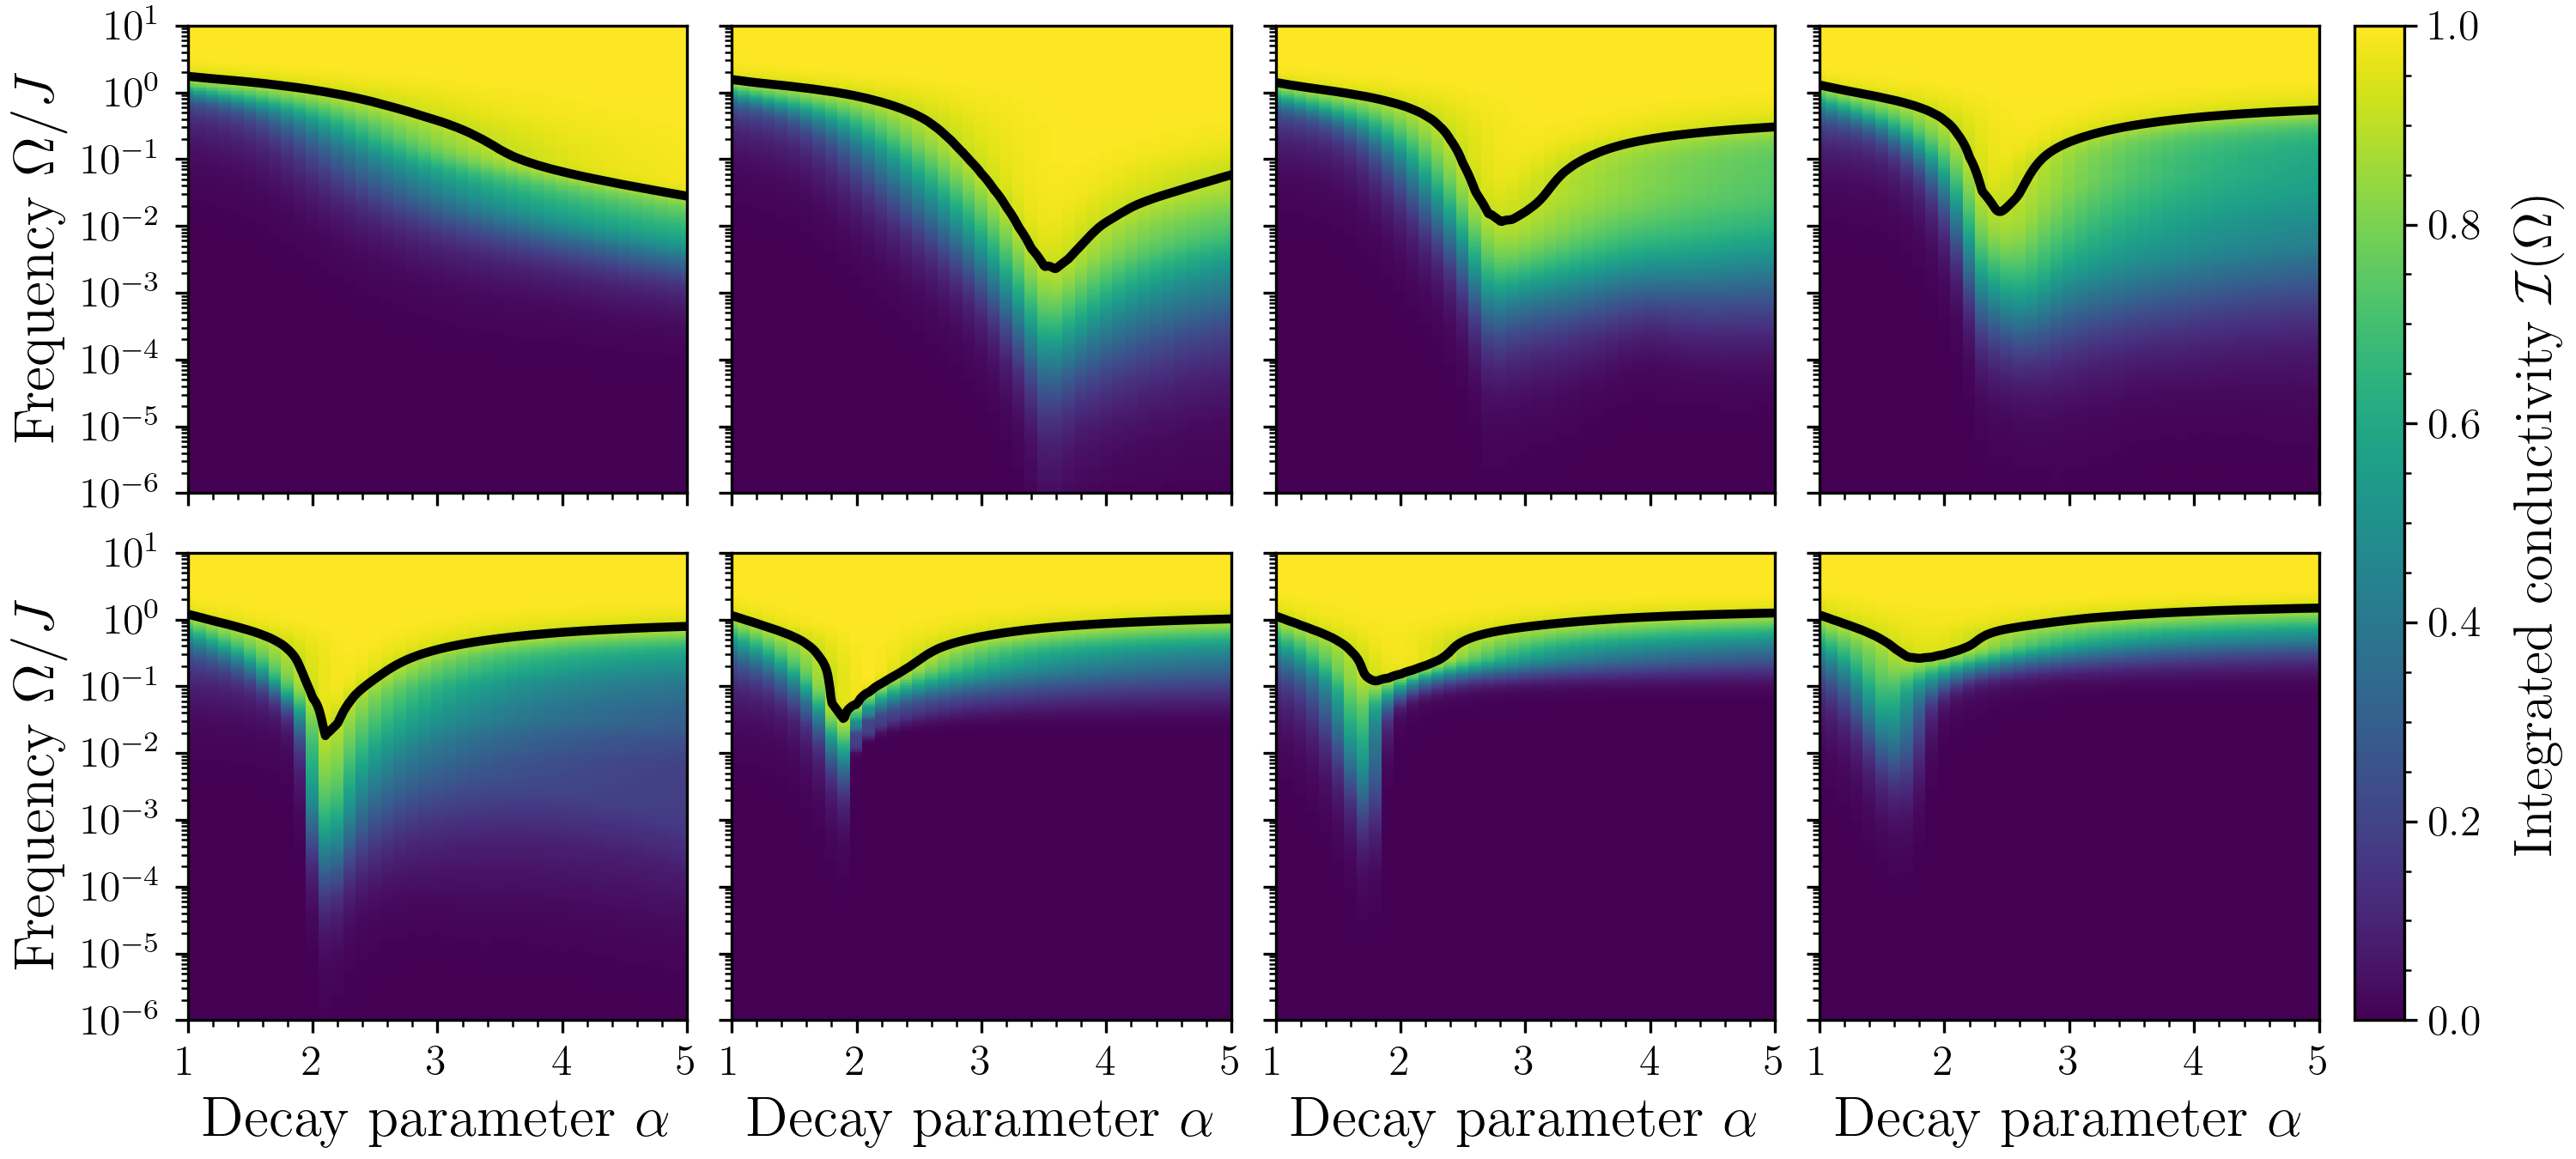
\includegraphics[width=\linewidth]{Figures/I_cond_heatmap.png}
  \caption{Heatmaps of the integrated conductivity \(I(\Omega)\) on the \((\alpha ,\Omega)\) plane.
  Black solid line denotes the value \(\Omega = \Omega^{\ast}\), 
  for which the integrated conductivity is \(I(\Omega^{\ast}) = 0.9\).}
  \label{fig:I_cond_heatmap}
\end{figure}

The results are presented in Fig.~\ref{fig:optimal_anisotropy}, and we observe an excellent
agreement between \(\Delta_{\sigma}\) obtained from linear response theory, that is low frequency (long time) dynamics,
of a system with periodic boundary conditions,
and the optimal anisotropy \(\Delta_{O}(\alpha)\), inferred from the short-time spin domain expansion in a chain
with open boundary conditions. This is a strong indication that the transient ballistic spin transport
is a generic feature of the long-range Heisenberg model, and not an artifact of the finite system size.
It is further supported by the finite-size analysis of the integrated conductivity, presented in the right panel
of Fig.~\ref{fig:optical_conductivity}, where we observe that \(I(\Omega)\) for \(\alpha = 2.0\)
is almost independent of the system size, and for larger values of \(\alpha\), the incoherent part of the spectrum
is shifted towards even lower frequencies.

\begin{figure}[htbp]
  \centering
  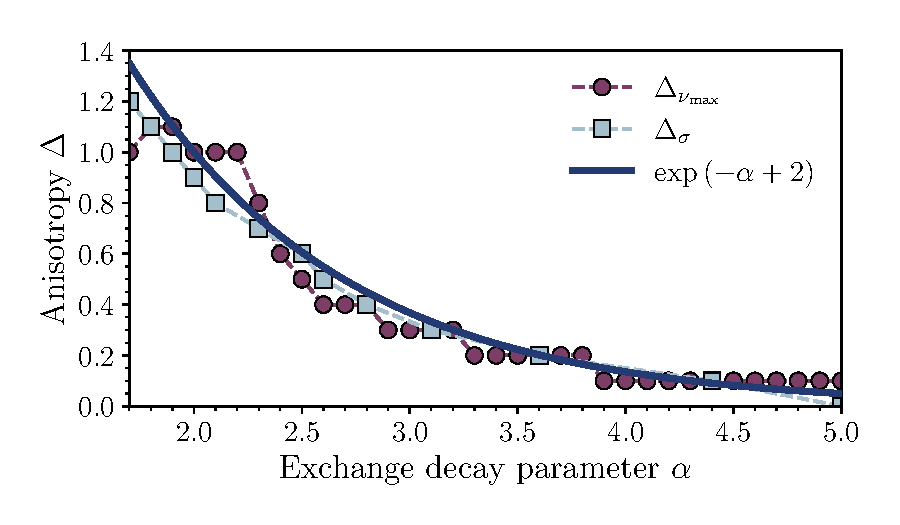
\includegraphics[width=0.8\linewidth]{Figures/optimal_anisotropies.pdf}
  \caption{Optimal values of anisotropy \(\Delta\), as a function of decay parameter \(\alpha\), obtained from
  the average velocity of spin expansion and integrated conductivity. The solid line denotes the optimal line
  \(\Delta_{\mathrm{O}} = \exp\left(-\alpha + 2\right)\).}
  \label{fig:optimal_anisotropy}
\end{figure}


It is worth mentioning, that in~\textcite{Mierzejewski2023},
we have also looked into a generalized version of the aforementioned Haldane-Shastry model,
with the exchange interaction of the form \(J_{\mathrm{HS}(\alpha)} \propto 1/\sin^{\alpha}(\pi r/L)\).
We have shown that it exhibits very similar behavior, with the integrated conductivity
close to the one obtained for the long-range Heisenberg model, and the optimal anisotropy
following the same exponential curve. Moreover, we have investigated two other
models, namely the next-nearest neighbor Heisenberg model (i.e.~\eqref{eq:long_range} with \(r_\mathrm{max} = 2\)),
and the long-range \(t\)-\(V\) spinless fermion model.
Contrary to the nearest-neighbor case, the long-range \(t\)-\(V\) model is not related to the long-range
Heisenberg model via the Jordan-Wigner transformation, and thus the two models are not equivalent.
The former case yielded results similar to the long-range Heisenberg model for small values
of anisotropy \(\Delta\in\left[0,0.2\right]\), while for larger values of \(\Delta\), the integrated conductivity
was rather featureless. It is consistent with our main results, as is this parameter regime, the optimal
decay is \(\alpha \gtrsim 3.5\), rendering the terms with \(r > 2\) insignificant.
In the latter case of spinless fermions, the quasibalistic transport was all but absent. Therefore,
it is expected that this phenomenon is unique to the long-range Heisenberg model.
For more details about those results, that go beyond the scope of this thesis, the interested reader is referred to
the original research article.
